\documentclass[11pt, spanish, letterpage]{article} %tipo de documento

\usepackage[letterpaper]{geometry} %margenes
\geometry{verbose,tmargin=2.5cm,bmargin=2.5cm,lmargin=2cm,rmargin=2cm}
\usepackage{amsmath,amsthm,amssymb} %modos matemáticos y  simbolos
\usepackage{latexsym,amsfonts} %simbolos matematicos
\usepackage{cancel} %hacer la linea que cancela las ecuaciones
\usepackage[spanish, es-noshorthands, es-nolayout]{babel} %comandos en español y cambia el cuadro por la tabla
\decimalpoint %cambia las comas por puntos decimal
\usepackage[utf8]{inputenc} %caracteristicas del español
\usepackage{physics} %Simbolos fisicos
\usepackage{array} %mejores formatos de tabla
\parindent =0cm %sangria
\usepackage{graphicx} %graficas e imagenes
\usepackage{mathtools}
\usepackage[framemethod=TikZ]{mdframed}%Entornos talegas
\usepackage[colorlinks = true,
			linkcolor = blue,
			citecolor = black,
			urlcolor = blue]{hyperref}%formato de los links y URL's
\usepackage{multicol} %varias columnas
\usepackage{enumerate} %enumeraciones
\usepackage{pgf,tikz,pgfplots} %documentos en formato tikz
\usepackage{mathrsfs} %letras chingonas (transformada de laplace)
\usepackage{subfigure} %varias figuras seguidas
\usepackage[square,numbers]{natbib} %bibliografias
\usepackage[nottoc]{tocbibind}
\bibliographystyle{plainnat}
\usetikzlibrary{arrows, babel, calc}
\usepackage{tabulary}
\usepackage{multirow} %ocupar varias filas en una tabla
\usepackage{fancybox} %recuadros talegas
\usepackage{float} %ubicar graficas
\usepackage{color}
\usepackage{comment}
\usepackage{stackrel}
\usepackage{calligra}
\usepackage{lipsum} % texto de relleno
\usepackage{cite}
\usepackage{circuitikz} % crear circuitos
\usepackage{listings} % permite el ingreso de codigo
\usepackage{longtable} % tablas a travez de paginas

\usepackage{fancyhdr}%formato de pagina
\pagestyle{fancy}%colocar la pagina con el formato deseado
\fancyhead{}
\fancyhead[L]{\footnotesize{Programación Matemática 1}}
\fancyhead[C]{Practica 1}
\fancyhead[R]{\footnotesize{\thepage}}
%\fancyhead[LO,RE]{Cálculo 3}
%\fancyhead[RO,LE]{\footnotesize{\thepage}}
\fancyfoot{}
\fancyfoot[L]{Diego Sarceño}
%\fancyfoot[LO,RE]{Diego Sarceño}
 
\begin{document} 
\begin{titlepage} 
% AUTOR: Diego Sarceño

% ENCABEZADO DE TRABAJOS CON LOGO DE LA UNIDAD ACADÉMICA

\begin{tabulary}{20cm}{Lp{0.9cm}p{6.1cm}}
Universidad de San Carlos de Guatemala & & \multirow{4}{8cm}{\hfill 
\includegraphics[scale=0.5]{ECFM.png}}\\            % Logo de la unidad academica
Escuela de Ciencias Físicas y Matemáticas & \hfill & \\
Diego Sarceño 201900109 & \hfill & \\
Programación Matemática 1 & \hfill & \\
\today & & \\
\end{tabulary}\\[0.25cm]

{\hrule height 1.5pt} \vspace{0.1cm}
\begin{tabulary}{21cm}{p{7cm}p{7cm}p{7cm}}
    \hfill & \huge{\scshape{Practica 1}} & \footnotesize{\scshape{Cuarto Semestre}}
\end{tabulary}
{\hrule height 1.5pt}
\vspace{0.5cm}

\section*{Datos}
\begin{longtable}{||c|c|c|p{4cm}||}
\hline 
\hline 
Cancion & Artista & Tiempo & Listas de reproduccion en las que aparece \\ 
\hline 
nombre & maje & 3.5 & q \\ 
\hline 
nombre & maje & 2.3 & p,q \\ 
\hline 
nombre & maje & 6 & p,q \\ 
\hline 
nombre & maje & 1 & p,q,r,s \\ 
\hline 
nombre & maje & 6 & p,q \\ 
\hline 
nombre & maje & 6.7 & p,q \\ 
\hline 
nombre & maje & 7.4 & p \\ 
\hline 
nombre & maje & 9.2 & p,q \\ 
\hline 
nombre & maje & 6.66 & p,q,r \\ 
\hline 
nombre & maje & 6.1 & q \\ 
\hline 
\hline 
\hline 
\end{longtable}
\section*{Grafica} 
\begin{figure}[H] 
\centering 
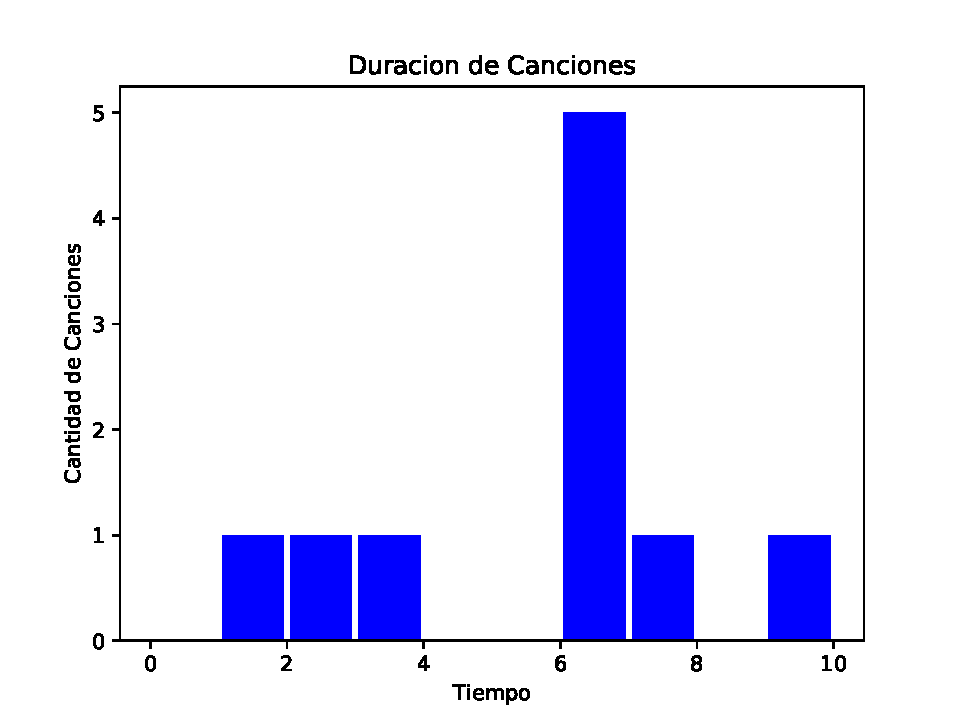
\includegraphics[scale=0.7]{histograma.pdf} 
\caption{Estadisticas} 
\end{figure} 
\end{titlepage}
\end{document}